%% Beginning of file 'sample701.tex'
%%
%% Version 7.0.1. Created May 2025.
%% Version 7. Created January 2025.  
%%
%% AASTeX v7+ calls the following external packages:
%% times, hyperref, ifthen, hyphens, longtable, xcolor, 
%% bookmarks, array, rotating, ulem, and lineno 
%%
%% RevTeX is no longer used in AASTeX v7+.
%%
\documentclass[apjl, linenumbers]{aastex701}
%%
%% This initial command takes arguments that can be used to easily modify 
%% the output of the compiled manuscript. Any combination of arguments can be 
%% invoked like this:
%%
%% \documentclass[argument1,argument2,argument3,...]{aastex701}
%%
%% Six of the arguments are typestting options. They are:
%%
%%  twocolumn   : two text columns, 10 point font, single spaced article.
%%                This is the most compact and represent the final published
%%                derived PDF copy of the accepted manuscript from the publisher
%%  default     : one text column, 10 point font, single spaced (default).
%%  manuscript  : one text column, 12 point font, double spaced article.
%%  preprint    : one text column, 12 point font, single spaced article.  
%%  preprint2   : two text columns, 12 point font, single spaced article.
%%  modern      : a stylish, single text column, 12 point font, article with
%% 		  wider left and right margins. This uses the Daniel
%% 		  Foreman-Mackey and David Hogg design.
%%
%% Note that you can submit to the AAS Journals in any of these 6 styles.
%%
%% There are other optional arguments one can invoke to allow other stylistic
%% actions. The available options are:
%%
%%   astrosymb    : Loads Astrosymb font and define \astrocommands. 
%%   tighten      : Makes baselineskip slightly smaller, only works with 
%%                  the twocolumn substyle.
%%   times        : uses times font instead of the default.
%%   linenumbers  : turn on linenumbering. Note this is mandatory for AAS
%%                  Journal submissions and revisions.
%%   trackchanges : Shows added text in bold.
%%   longauthor   : Do not use the more compressed footnote style (default) for 
%%                  the author/collaboration/affiliations. Instead print all
%%                  affiliation information after each name. Creates a much 
%%                  longer author list but may be desirable for short 
%%                  author papers.
%% twocolappendix : make 2 column appendix.
%%   anonymous    : Do not show the authors, affiliations, acknowledgments,
%%                  and author contributions for dual anonymous review.
%%  resetfootnote : Reset footnotes to 1 in the body of the manuscript.
%%                  Useful when there are a lot of authors and affiliations
%%		    in the front matter.
%%   longbib      : Print article titles in the references. This option
%% 		    is mandatory for PSJ manuscripts.
%%
%% Since v6, AASTeX has included \hyperref support. While we have built in 
%% specific %% defaults into the classfile you can manually override them 
%% with the \hypersetup command. For example,
%%
%% \hypersetup{linkcolor=red,citecolor=green,filecolor=cyan,urlcolor=magenta}
%%
%% will change the color of the internal links to red, the links to the
%% bibliography to green, the file links to cyan, and the external links to
%% magenta. Additional information on \hyperref options can be found here:
%% https://www.tug.org/applications/hyperref/manual.html#x1-40003
%%
%% The "bookmarks" has been changed to "true" in hyperref
%% to improve the accessibility of the compiled pdf file.
%%
%% If you want to create your own macros, you can do so
%% using \newcommand. Your macros should appear before
%% the \begin{document} command.
%%
\newcommand{\vdag}{(v)^\dagger}
\newcommand\aastex{AAS\TeX}
\newcommand\latex{La\TeX}
%%%%%%%%%%%%%%%%%%%%%%%%%%%%%%%%%%%%%%%%%%%%%%%%%%%%%%%%%%%%%%%%%%%%%%%%%%%%%%%%
%%
%% The following section outlines numerous optional output that
%% can be displayed in the front matter or as running meta-data.
%%
%% Running header information. A short title on odd pages and 
%% short author list on even pages. Note that this
%% information may be modified in production.
%%\shorttitle{AASTeX v7.0.1 Sample article}
%%\shortauthors{The Terra Mater collaboration}
%%
%% Include dates for submitted, revised, and accepted.
%%\received{February 1, 2025}
%%\revised{March 1, 2025}
%%\accepted{\today}
%%
%% Indicate AAS Journal the manuscript was submitted to.
%%\submitjournal{PSJ}
%% Note that this command adds "Submitted to " the argument.
%%
%% You can add a light gray and diagonal water-mark to the first page 
%% with this command:
%% \watermark{text}
%% where "text", e.g. DRAFT, is the text to appear.  If the text is 
%% long you can control the water-mark size with:
%% \setwatermarkfontsize{dimension}
%% where dimension is any recognized LaTeX dimension, e.g. pt, in, etc.
%%%%%%%%%%%%%%%%%%%%%%%%%%%%%%%%%%%%%%%%%%%%%%%%%%%%%%%%%%%%%%%%%%%%%%%%%%%%%%%%
%%
%% Use this command to indicate a subdirectory where figures are located.
%%\graphicspath{{./}{figures/}}
%% This is the end of the preamble.  Indicate the beginning of the
%% manuscript itself with \begin{document}.
\usepackage{siunitx}
\usepackage{float}
\begin{document}

\title{Template \aastex v7.0.1 Article with Examples\footnote{Footnotes can be added to titles}}

%% A significant change from AASTeX v6+ is in the author blocks. Now an email
%% address is required for each author. This means that each author requires
%% at least one of the following:
%%
%% \author
%% \affiliation
%% \email
%%
%% If these three commands are not available for each author, the latex
%% compiler will issue an error and if you force the latex compiler to continue,
%% it will generate an incomplete pdf.
%%
%% Multiple \affiliation commands are allowed and authors can also include
%% an optional \altaffiliation to indicate a status, i.e. Hubble Fellow. 
%% while affiliations are indexed as footnotes, altaffiliations are noted with
%% with a non-numeric footnote that is set away from the numeric \affiliation 
%% footnotes. NOTE that if an \altaffiliation command is used it must 
%% come BEFORE the \affiliation call, right after the \author command, in 
%% order to place the footnotes in the proper location. Because non-numeric
%% symbols are used, \altaffiliation should be used sparingly.
%%
%% In v7+ the \author command takes an optional argument which provides 
%% additional metadata about the author. Authors can provide the 16 digit 
%% ORCID, the surname (family or last) name, the given (first or fore-) name, 
%% and a name suffix, e.g. "Jr.". The syntax is:
%%
%% \author[orcid=0000-0002-9072-1121,gname=Gregory,sname=Schwarz]{Greg Schwarz}
%%
%% This name metadata in not shown, it is only for parsing by the peer review
%% system so authors can be more easily identified. This name information will
%% also be sent to the publisher so they can include it in the CROSSREF 
%% metadata. Including an orcid will hyperlink the author name to the 
%% author's ORCID page. Note that  during compilation, LaTeX will do some 
%% limited checking of the format of the ID to make sure it is valid. If 
%% the "orcid-ID.png" image file is  present or in the LaTeX pathway, the 
%% ORCID icon will appear next to the authors name.
%%
%% Even though emails are now required for each author, the \email does not
%% produce output in the compiled manuscript unless the optional "show" command
%% is used. For example,
%%
%% \email[show]{greg.schwarz@aas.org}
%%
%% All "shown" emails are show in the bottom left of the first page. Due to
%% space constraints, only a few emails should be shown. 
%%
%% To identify a corresponding author, use the \correspondingauthor command.
%% The command appends "Corresponding Author: " to the argument it appears at
%% the bottom left of the first page like the output from \email. 

\author[orcid=0000-0000-0000-0001,sname='Mehta']{Shreyansh Mehta}
\altaffiliation{}
\affiliation{Indian Institute of Technology, Kanpur}
\email[show]{shreyanshm24@iitk.ac.in}  

\author[orcid=0000-0000-0000-0002,gname=Bosque, sname='Sur America']{Forrest Sur Am\'{e}rica} 
\altaffiliation{Las Campanas Observatory}
\affiliation{Universidad de Chile, Department of Astronomy}
\email{fakeemail2@google.com}

\author[gname=Savannah,sname=Africa]{S. Africa}
\affiliation{South African Astronomical Observatory}
\affiliation{University of Cape Town, Department of Astronomy}
\email{fakeemail3@google.com}

\author{River Europe}
\affiliation{University of Heidelberg}
\email{fakeemail4@google.com}

\author[0000-0000-0000-0003,sname=Asia,gname=Mountain]{Asia Mountain}
\altaffiliation{Astrosat Post-Doctoral Fellow}
\affiliation{Tata Institute of Fundamental Research, Department of Astronomy}
\email{fakeemail5@google.com}

\author[0000-0000-0000-0004]{Coral Australia}
\affiliation{James Cook University, Department of Physics}
\email{fakeemail6@google.com}

\author[gname=IceSheet]{Penguin Antarctica}
\affiliation{Amundsen–Scott South Pole Station}
\email{fakeemail7@google.com}

\collaboration{all}{The Terra Mater collaboration}

%% Use the \collaboration command to identify collaborations. This command
%% takes an optional argument that is either a number or the word "all"
%% which tells the compiler how many of the authors above the command to
%% show. For example "\collaboration[all]{(DELVE Collaboration)}" wil include
%% all the authors above this command.
%%
%% Mark off the abstract in the ``abstract'' environment. 
\begin{abstract}

This example manuscript is intended to serve as a tutorial and template for
authors to use when writing their own AAS Journal articles. The manuscript
includes a history of \aastex\ and documents the new features in the
previous versions as well as the new features in version 7. This
manuscript includes many figure and table examples to illustrate these new
features.  Information on features not explicitly mentioned in the article
can be viewed in the manuscript comments or more extensive online
documentation. Authors are welcome replace the text, tables, figures, and
bibliography with their own and submit the resulting manuscript to the AAS
Journals peer review system.  The first lesson in the tutorial is to remind
authors that the AAS Journals, the Astrophysical Journal (ApJ), the
Astrophysical Journal Letters (ApJL), the Astronomical Journal (AJ), and 
the Planetary Science Journal (PSJ) all have a 250 word limit for the 
abstract. The limit is 150 for RNAAS manuscripts. If you exceed this length 
the Editorial office will ask you to shorten it. This abstract has 189 words.

\end{abstract}

%% Keywords should appear after the \end{abstract} command. 
%% The AAS Journals now uses Unified Astronomy Thesaurus (UAT) concepts:
%% https://astrothesaurus.org
%% You will be asked to selected these concepts during the submission process
%% but this old "keyword" functionality is maintained in case authors want
%% to include these concepts in their preprints.
%%
%% You can use the \uat command to link your UAT concepts back its source.
\keywords{\uat{Galaxies}{573} --- \uat{Cosmology}{343} --- \uat{High Energy astrophysics}{739} --- \uat{Interstellar medium}{847} --- \uat{Stellar astronomy}{1583} --- \uat{Solar physics}{1476}}

%% From the front matter, we move on to the body of the paper.
%% Sections are demarcated by \section and \subsection, respectively.
%% Observe the use of the LaTeX \label
%% command after the \subsection to give a symbolic KEY to the
%% subsection for cross-referencing in a \ref command.
%% You can use LaTeX's \ref and \label commands to keep track of
%% cross-references to sections, equations, tables, and figures.
%% That way, if you change the order of any elements, LaTeX will
%% automatically renumber them.

\section{Introduction}  \label{sec:intro}

Fast radio bursts (FRBs) are millisecond-duration radio transients of extragalactic origin \citep{LorimerFirstFRB}. Although magnetars have emerged as leading progenitor candidates \citep{CHIME2020, MagnetarFRB2}, the origin of the broader FRB population remains unknown. With a growing number of FRBs localized to arcsecond precision, the demographics of FRB host galaxies and their local environments \citep{Gordon2023} have become one of the main tools to address this problem. Such studies, however, may be biased by selection effects that make FRBs harder to detect for certain hosts.

The host galaxy itself can affect whether an FRB is detected. A burst from a source embedded in a galactic disk must propagate through the ionized interstellar medium of its host, which adds to its dispersion measure (DM) and broadens it through scattering \citep{xuHan2015, Ocker2022}. Both effects grow with the path length through the disk, and are therefore expected to be larger in hosts viewed edge-on \citep{xuHan2015, Orr2024}, which could lead to a potential selection bias against detecting FRBs in edge-on hosts. 

\citet{Bhardwaj2024} provided the first empirical test of this idea, finding that the inclination angles of 23 FRB hosts from untargeted surveys are skewed toward lower inclination angles (face-on) compared with SDSS field galaxies. Their inclination angles were derived from profile fits to ground-based imaging that did not include the point spread function (PSF), which is well suited to resolved galaxies. Many FRB hosts, however, are only marginally resolved in archival imaging, and seeing circularizes such galaxies, which raises the projected axis ratio, $q = b/a$, and makes the inferred inclination angle appear more face-on \citep{Trujillo2001}. PSF-aware profile fits can therefore help separate a genuine edge-on deficit from the effect of PSF circularization.

In this study, we revisit the inclination distribution of FRB hosts with two additions. First, we expand the sample to 56 hosts of FRBs discovered by untargeted surveys, more than twice that of \citet{Bhardwaj2024} and including 22 of their 23 hosts. Second, we construct an empirical PSF model for each field, fit two-dimensional S\'ersic profiles convolved with the PSF, and convert the recovered $q$ to an inclination angle. We compare these inclinations with those of disk galaxies from the Hyper Suprime-Cam Subaru Strategic Program (HSC-SSP) structural catalog \citep{Kawinwanichakij}, whose axis ratios are measured with the same class of PSF-convolved model. We find that the inclination distribution of FRB hosts is consistent with that of field disk galaxies, and we do not recover a deficit of edge-on hosts. The original 23 hosts of \citet{Bhardwaj2024}, remeasured with PSF-convolved fits, are also consistent with the field galaxies, which suggests that the treatment of the PSF accounts for most of the difference between the two studies.

We describe the sample and inclination measurements in Section~\ref{sec:methods}, present our results in Section~\ref{sec:results}, and discuss their implications in Section~\ref{sec:discussion}.

\section{Methodology} \label{sec:methods}
\subsection{Sample and Imaging Data} \label{sec:sample}

We select published FRBs localized with arcsecond precision. To avoid biases from targeted searches, we include only FRBs discovered by untargeted surveys. Most events come from the Commensal Real-time ASKAP Fast Transients (CRAFT) survey \citep{CRAFT} and the Deep Synoptic Array-110 (DSA-110) \citep{DSA110}, with additional events from the More Transients and Pulsars with MeerKAT (MeerTRAP) survey \citep{MeerTrap}, the Deep Synoptic Array ten-antenna prototype (DSA-10) \citep{DSA10}, and the Canadian Hydrogen Intensity Mapping Experiment (CHIME) Outriggers \citep{CHIMEOutriggers}. [Repeaters: included or excluded, and why. Since 20220912A seems to be a repeater but is also in the original 23?]

We use imaging from the Dark Energy Spectroscopic Instrument (DESI) Legacy Imaging Surveys (LS) DR10 \citep{Desi} and the Panoramic Survey Telescope and Rapid Response System (Pan-STARRS) DR1 \citep{PS1}, which are sensitive down to apparent $r$-band magnitudes ($m_r$) of approximately 23.5 and 22 AB mag, respectively. We prioritize LS data for their greater depth, using Pan-STARRS only for hosts outside the LS footprint. For one host, FRB~20240208A, we use deeper HSC-SSP PDR2 Wide $r$-band imaging \citep{HS-SCSSP}, retrieved through the CDS HiPS service \citep{Fernique2015} and resampled to the LS pixel scale of $0.262\arcsec$~pixel$^{-1}$. To ensure robust inclination measurements from archival imaging, we restrict the sample to hosts with $m_r \leq 22$ AB mag. All Pan-STARRS hosts in our sample have $m_r \leq 20.1$ AB mag, about 2 mag brighter than the survey limit. Two further hosts are excluded because no stable axis ratio could be recovered: FRB~20221101B lies $6\arcsec$ from a bright foreground star whose light could not be modeled or masked without affecting the host within $\sim R_e$ \citep[as in][]{Japelij2018}, and FRB~20230930A lies on structured diffuse emission that prevents a reliable sky model. [Maybe assign either host face-on and edge-on and see if the results change significantly] This yields 63 FRB hosts, listed in Table~1, of which 56 remain after the axis-ratio cut described in Section~\ref{sec:inclination}.

\subsection{Estimating Inclination Angles} \label{sec:inclination}

To estimate the inclination angle $i$ of each host, defined as the angle between the normal to the galactic disk and our line of sight (such that $i = \ang{0}$ is face-on and $i = \ang{90}$ is edge-on), we fit parametric profiles using \texttt{GALFIT} \citep{Galfit, Galfit2}. We detect sources in a $10\arcmin \times 10\arcmin$ field centered on each host with \texttt{Source Extractor} \citep{SExtractor}, and run \texttt{PSFEx} \citep{PSFEx} on the resulting catalog to build an empirical PSF model for each field. For the HSC-SSP host, the PSF is built from the resampled HiPS image. Initial parameters for the \texttt{GALFIT} fits are taken from a second, PSF-aware \texttt{Source Extractor} run. We fit each host simultaneously with neighboring extended sources that could contaminate its light profile, modeling each as an independent S\'ersic component, and mask stars beyond $\sim R_e$ and model those within it with a PSF component. We also use \texttt{statmorph} \citep{Statmorph} to perform a non-parametric analysis of the hosts as a diagnostic.

The formal uncertainties reported by \texttt{GALFIT} are known to underestimate the true parameter uncertainties \citep{Haussler2007, Galfit2}. Significant additional contributions to the uncertainty in $q$ come from mismatch between the model and the true light distribution of the galaxy \citep{Galfit2} and from errors in the sky level \citep{Haussler2007, Gao2017}. We account for the former through a systematic term on $i$ (see below), and for the latter by adding to the formal uncertainty on $q$, in quadrature, a sky term $\sigma_{q,\mathrm{sky}}$. Following the approach of \citet{Huang2013} and \citet{Gao2017}, we obtain this term by refitting each host with the sky fixed at $s_0 \pm \sigma_{\mathrm{sky}}$, where $s_0$ is the best-fitting sky level and $\sigma_{\mathrm{sky}}$ is the scatter of local background estimates across the field, and taking half the difference between the two resulting values of $q$.

We convert axis ratios to inclination angles using the Hubble formula \citep{Hubble}, which treats a disk as an oblate spheroid with intrinsic axis ratio $q_0$:

\begin{equation} \label{eq:HubbleFormula}
\cos^2 i = \frac{q^2 - q_0^2}{1 - q_0^2}. 
\end{equation}

Following \citet{Bhardwaj2024}, we adopt $q_0 = 0.2$
\citep{vandenBergh1988}. We note that our results are insensitive to this choice (Appendix~\ref{app:q0}). Equation~\ref{eq:HubbleFormula} is undefined for $q < q_0$, and, following \citet{Japelij2018}, we exclude such hosts, since inclinations near this limit are highly uncertain. Seven of the 63 hosts have $q \leq 0.2$, leaving a final sample of 56.

We propagate $\sigma_q$ through Equation~\ref{eq:HubbleFormula} by Monte Carlo sampling to obtain $\sigma_{i,q}$, and add a systematic term of \ang{5} in quadrature, 

\begin{equation} \label{eq:InclinationSystematic}
\sigma_i^2 = \sigma_{i,q}^2 + (\ang{5})^2.
\end{equation}

This term accounts for errors that a single S\'ersic model does not capture: non-axisymmetric structure such as bars and spiral arms introduces inclination uncertainties of $\approx\ang{5}$ on average \citep{Barnes2003}, and further errors may arise from intrinsic non-circularity of disks \citep{Ryden2004} and variations in disk thickness around $q_0$. [Optional: The RMS difference between our \texttt{GALFIT} and \texttt{statmorph} inclinations, X\arcdeg, is comparable to this term.] 

\subsection{Null Hypothesis} \label{sec:control}

If FRB detectability does not depend on host orientation, FRB hosts should share the inclination distribution of field disk galaxies. Since the Universe is statistically isotropic \citep{Saadeh2016} and alignments between galaxies are weak \citep{Joachimi2015J}, there is no preferred orientation for galactic disks, which corresponds to a uniform distribution in $\cos i$. However, measured inclinations deviate from this uniformity due to the limitations inherent in the methods used to estimate $i$. We therefore compare the FRB hosts with field galaxies whose inclinations are measured in a comparable way, rather than with a uniform distribution.

We draw this control sample from the HSC-SSP structural catalog \citep{Kawinwanichakij}, which provides axis ratios from PSF-convolved single-S\'ersic fits with the S\'ersic index $n$ left free, the same model class we fit to the FRB hosts, and report that these measurements are consistent with \texttt{GALFIT} fits. These fits use the HSC i band rather than $r$; since single-band fits show no significant variation of the axis ratio across the optical bands \citep{Vika2013}, this should have little effect on our comparison. We select galaxies with \texttt{goodfits\_flag}~$=1$ and apply the same magnitude limit ($r \leq 22$ AB mag) and axis-ratio cut ($q > 0.2$) as for the FRB hosts. Since our FRB hosts are disk-dominated (Appendix~\ref{app:morph}), we exclude early-type systems by retaining only galaxies with $0.4 < n < 1.5$. This yields 24{,}450 galaxies, whose axis ratios we convert to inclinations using Equation~\ref{eq:HubbleFormula}. Our conclusions are insensitive to these selection criteria (Appendix~\ref{app:morph}).

\section{Analysis} \label{sec:results}

Figure~\ref{fig:cdf}a shows the cumulative distribution functions (CDFs) of $\cos i$ for the 56 FRB hosts and the control sample. Following \citet{Bhardwaj2024}, we account for sampling effects by drawing 10{,}000 random samples of 56 galaxies from the control sample, and show the 68\% bound of these realizations in Figure~\ref{fig:cdf}a. For each test below, we quote $p_{\rm m}$, the fraction of these realizations that differ from the control sample at least as much as the FRB hosts do. The FRB hosts have a median $\cos i$ of 0.626 ($i \approx \ang{51.3}$), compared with 0.575 ($i \approx \ang{54.9}$) for the control sample.
 
To compare the two distributions, we use the two-sample Anderson--Darling (AD) test \citep{KS-AD} and the Mann--Whitney (MW) $U$ test \citep{MW}, as in \citet{Bhardwaj2024}. Run two-sided, these give $p_{\rm m} = 0.54$ (AD) and $p_{\rm m} = 0.46$ (MW); for reference, \citet{Bhardwaj2024} found $p = 0.0003$ and $p = 0.00012$ against SDSS. To test specifically for a deficit of edge-on hosts, we also run the MW test one-sided in that direction, which gives $p_{\rm m} = 0.23$. None of these tests indicates a significant difference, and the inclination distribution of our FRB hosts is consistent with that of field disk galaxies. The same holds for the 23 hosts of \citet{Bhardwaj2024} alone once remeasured with our PSF-convolved fits (Figure~\ref{fig:cdf}b; AD $p_{\rm m} = 0.93$, two-sided MW $p_{\rm m} = 0.84$, one-sided MW $p_{\rm m} = 0.42$). We note that neither result is a consequence of limited sensitivity. For each sample
size, we draw 2{,}000 samples, with replacement, from the 23 published
inclinations of \citet{Bhardwaj2024}; the AD test detects their reported
deficit ($p < 0.05$) in more than 99\% of samples of 56 hosts and in 91\%
of samples of 23. Rerunning the \texttt{AstroPhot} \citep{Astrophot} fits of \citet{Bhardwaj2024} with PSF convolution gives inclinations consistent with ours (RMS difference $\approx \ang{5}$; Figure~\ref{fig:cdf}b), while our fits without the PSF closely reproduce their published values (RMS difference \ang{3.4}; Appendix~\ref{app:psf}). This suggests that the difference between the two results arises mainly from the treatment of the PSF, rather than from the sample or the imaging.

\begin{figure}[H]
\centering
\includegraphics[width=\textwidth]{fig1_cdf.pdf}
\caption{CDFs of $\cos i$. (a) The 56 FRB hosts (red) and the control sample (blue), with the 68\% bound of 10{,}000 random samples of 56 control galaxies (shaded). (b) The 23 hosts of \citet{Bhardwaj2024}, using their published inclinations (grey) and our PSF-convolved remeasurements with \texttt{GALFIT} (red) and \texttt{AstroPhot} (orange), with the 68\% bound for samples of 23. The dashed line shows a uniform distribution.}
\label{fig:cdf}
\end{figure}

Following \citet{Bhardwaj2024}, we also divide the control sample into four bins corresponding to the quartiles of its $\cos i$ distribution, so that each bin is expected to contain 14 of the 56 FRB hosts. From face-on to edge-on, the FRB hosts are distributed across these bins as 14, 19, 10, and 13 (Figure~\ref{fig:bins}; $p_{\rm m} = 0.40$). The most face-on bin ($i < \ang{41.0}$) and the most edge-on bin ($i > \ang{67.1}$) contain 14 and 13 hosts, respectively, close to the expected 14. For comparison, \citet{Bhardwaj2024} found 11 of their 23 hosts in the most face-on bin and one in the most edge-on bin, from which they estimated that FRB rates may be underestimated by a factor of two. With PSF-convolved inclinations, we find no excess of face-on hosts and no deficit of edge-on hosts, so a correction of this size does not appear to be needed. Including measurement uncertainties does not change these conclusions (Appendix~\ref{app:errors}).

\begin{figure}[H]
\centering
\includegraphics[width=\textwidth]{fig2_bins.pdf}
\caption{Number of FRB hosts in each of four inclination bins, defined by the quartiles of the control sample's $\cos i$ distribution; the bin ranges are marked on the horizontal axis. The dashed line marks the expected 14 hosts per bin, and the shaded band the 68\% range from random samples of 56 control
galaxies.}
\label{fig:bins}
\end{figure}

Even without a detection bias, a longer path through the host disk could
raise the DM and scattering of bursts in inclined hosts, and
\citet{marnoch2026} reported that the rest-frame DM$_{\rm host}$ of 34 CRAFT
FRBs decreases with the axis ratio of their hosts ($r_S = -0.44$). We test
for such a trend using the 55 hosts with spectroscopic redshifts
(Figure~\ref{fig:corr}). Since every host has $q > q_0$, $\cos i$ is a
monotonic function of $q$, and rank correlations with either are identical.
We find no significant correlation between DM$_{\rm host}$ and $q$ (Spearman
$r_S = -0.06$, $p = 0.64$; Kendall $\tau = -0.04$, $p = 0.63$;
\citealt{Kendall1938}; Figure~\ref{fig:corr}a). To guard against outliers, we
also compute bootstrap confidence intervals \citep{Efron1979}, jackknife
values with one to three hosts removed, and the Theil--Sen slope
\citep{Sen1968}. The bootstrap 95\% interval is $-0.32 < r_S < 0.20$;
removing any one host keeps $r_S$ between $-0.12$ and $-0.04$, and removing
any two or three keeps it between $-0.21$ and $+0.02$, with $p > 0.13$ in
every case; and the Theil--Sen slope, $-38^{+197}_{-201}$~pc~cm$^{-3}$ per
unit $q$, is consistent with zero. Since a rank correlation tests only for a
monotonic trend, we also compare the DM$_{\rm host}$ distributions of the
more face-on and more edge-on halves of the sample with the AD test, which
finds no difference ($p = 0.18$). The result is unchanged for hosts with
$m_r < 21$ or $n < 2$, or without the three hosts that \citet{marnoch2026} fit
with a bulge component, and when we subtract the DM contributed by foreground
galaxy halos along each sightline (Figure~\ref{fig:corr}b;
Appendix~\ref{app:halo}). Our axis ratios agree closely with those of
\citet{marnoch2026} for the 20 hosts in both samples
(Appendix~\ref{app:marnoch}), so the difference is unlikely to come from the
inclination measurements. Combining the two samples into 69 unique hosts,
with their DM$_{\rm host}$ values placed on our definition, roughly halves the
correlation, to $r_S = -0.21$ ($p = 0.08$) with our values for the shared hosts
and $r_S = -0.22$ ($p = 0.07$) with theirs, and to $r_S = -0.16$ to $-0.17$
($p = 0.17$ to 0.20) for the hosts with $q > q_0$. This suggests that the trend in the smaller
sample may partly reflect sample variance, together with differences in
sample selection between the two studies. None of the other burst properties we compiled from the literature
correlates significantly with inclination: $|{\rm RM}|$ ($r_S = -0.02$,
$p = 0.91$, $N = 41$), scattering time ($r_S = -0.17$, $p = 0.39$, $N = 29$),
and linear polarization fraction ($r_S = -0.33$, $p = 0.11$, $N = 24$),
although the two smaller samples cannot exclude a moderate trend. The extinction of the older
stellar population increases toward edge-on ($r_S = -0.46$, $p = 0.010$;
$p_{\rm AD} = 0.005$; $N = 30$), as expected for dust in inclined disks, and
remains at $p < 0.05$ after removing any one host and in at least 97\% of
cases with two or three removed. It is, however, not
significant after correcting for the 41 host and burst properties tested
\citep{BH1995}. The same compiled values recover the known correlations of
DM$_{\rm host}$ with scattering time ($r_S = 0.45$, $p = 0.014$) and
$|{\rm RM}|$ ($r_S = 0.49$, $p = 0.001$), so the compiled properties are
precise enough to reveal such trends.

\begin{figure}[H]
\centering
\includegraphics[width=\textwidth]{fig3_correlations.pdf}
\caption{Host and burst properties versus host axis ratio. (a) Rest-frame
DM$_{\rm host}$ for the 55 FRB hosts with spectroscopic redshifts (filled), and
after subtracting the DM of intersected foreground halos for the 49 hosts in
the LS footprint (open; Appendix~\ref{app:halo}), with lines joining the two
values. The solid line and shaded band show the Theil--Sen fit to the filled
points and the 95\% range of its slope. (b) Spearman $r_S$ with bootstrap 95\%
confidence intervals for DM$_{\rm host}$ in the full sample, after removing the
total or the excess foreground halo contribution, and in subsamples (red), and
for other host and burst properties (blue). The Spearman $p$-value is given in
parentheses beside each point, and filled symbols have $p < 0.05$. The columns
at right give the number of hosts and the AD $p$-value comparing the hosts
above and below the median $q$.}
\label{fig:corr}
\end{figure}

\section{Conclusions} \label{sec:conclusions}

%% Please use the acknowledgment and contribution environments. This will 
%% be anonomyized when the "anonymous" style option is used. 

% TODO: give the bin edges in note b to two decimals, computed from the unrounded
% quartiles. FRB 20240318A (67.14 deg, bin 3) sits on the 67.1 deg edge.
% TODO: the inclinations repeat exactly (e.g. 69.30 three times, 52.43 four times)
% because they were computed from q rounded to 0.01. Recompute from full-precision q.
\startlongtable
\begin{deluxetable*}{rlccccccccl}
\tabletypesize{\scriptsize}
\tablecolumns{11}
\tablewidth{0pt}
\tablecaption{FRB host galaxies considered in this work\label{tab:sample57}}
\tablehead{
\colhead{No.\tablenotemark{a}} & \colhead{FRB} & \colhead{$i$\tablenotemark{b}} & \colhead{Bin} & \colhead{SFR\tablenotemark{c}} & \colhead{$\log({\rm sSFR})$} & \colhead{Mass} & \colhead{$z$} & \colhead{DM$_{\rm host}$} & \colhead{Host $m_r$\tablenotemark{d}} & \colhead{Ref.} \\
\colhead{} & \colhead{} & \colhead{(deg)} & \colhead{} & \colhead{($M_\odot$\,yr$^{-1}$)} & \colhead{(yr$^{-1}$)} & \colhead{($10^{10}\,M_\odot$)} & \colhead{} & \colhead{(pc\,cm$^{-3}$)} & \colhead{(AB mag)} & \colhead{}
}
\startdata
\textbf{1} & 20171020A & 69.30 & 4 & 0.09$^{\dagger}$ & $-9.69$ & 0.04 & 0.0087 & 70 & 15.10 & 1 \\
2 & 20180924B & 48.45 & 2 & 0.62 & $-10.60$ & 2.45 & 0.3214 & 62 & 20.24 & 2, 3 \\
3 & 20181112A & 31.14 & 1 & 1.54 & $-9.68$ & 0.74 & 0.4755 & 187 & 21.98 & 2, 3 \\
4 & 20190102C & 73.17 & 4 & 0.40 & $-10.09$ & 0.49 & 0.2912 & 79 & 21.67 & 2, 3 \\
5 & 20190523A & 44.70 & 2 & $<1.30$ & $<-10.96$ & 11.75 & 0.6600 & 196 & 21.72 & 4 \\
6 & 20190608B & 46.79 & 2 & 7.03 & $-9.71$ & 3.63 & 0.1178 & 235 & 17.46 & 2, 3 \\
7 & 20190714A & 69.30 & 4 & 1.89 & $-9.94$ & 1.66 & 0.2365 & 333 & 20.24 & 2, 3 \\
8 & 20191001A & 59.21 & 3 & 18.28 & $-9.47$ & 5.37 & 0.2340 & 332 & 18.41 & 2, 3 \\
9 & 20200906A & 73.70 & 4 & 4.93 & $-9.68$ & 2.34 & 0.3688 & 305 & 20.13 & 2, 3 \\
10 & 20210320C & 46.79 & 2 & 3.51 & $-9.82$ & 2.34 & 0.2797 & 137 & 19.80 & 2, 3 \\
11 & 20210410D & 69.99 & 4 & 0.03 & $-10.99$ & 0.30 & 0.1415 & 468 & 21.12 & 2, 5 \\
\textbf{12} & 20210807D & 45.92 & 2 & 0.63 & $-11.17$ & 9.33 & 0.1293 & 33 & 15.93 & 2, 3 \\
\textbf{13} & 20211127I & 13.52 & 1 & 35.83 & $-7.93$ & 0.30 & 0.0469 & 164 & 14.25 & 2, 3 \\
14 & 20211203C & 23.58 & 1 & 15.91 & $-8.56$ & 0.58 & 0.3439 & 373 & 20.11 & 2, 3 \\
15 & 20211212A & 34.70 & 1 & 0.73 & $-10.42$ & 1.91 & 0.0707 & 134 & 16.46 & 2, 3 \\
\textbf{16} & 20220207C & 83.34 & 4 & 0.71 & $-10.10$ & 0.89 & 0.0433 & 157 & 18.12 & 6 \\
\textbf{17} & 20220307B & 52.43 & 2 & 3.17 & $-9.64$ & 1.38 & 0.2481 & 196 & 19.87 & 6 \\
18 & 20220310F & 47.62 & 2 & 0.97 & $-9.99$ & 0.95 & 0.4780 & $-12$ & 20.83 & 6 \\
\textbf{19} & 20220319D & 37.76 & 1 & 0.42 & $-10.48$ & 1.26 & 0.0112 & $-31$ & 16.08 & 6 \\
20 & 20220418A & 41.55 & 2 & 1.31 & $-10.14$ & 1.82 & 0.6214 & 30 & 20.88 & 6 \\
21 & 20220501C & 58.78 & 3 & \nodata & \nodata & \nodata & 0.3810 & 121 & 21.80 & 3 \\
22 & 20220509G & 58.94 & 3 & 0.25 & $-11.30$ & 5.01 & 0.0894 & 158 & 16.66 & 6 \\
23 & 20220725A & 54.85 & 2 & 10.73$^{\dagger}$ & $-9.67$ & 5.01 & 0.1926 & 122 & 17.76 & 7, 3 \\
\textbf{24} & 20220825A & 53.20 & 2 & 7.91 & $-9.11$ & 1.02 & 0.2414 & 461 & 19.98 & 6 \\
25 & 20220914A & 61.39 & 3 & 0.46 & $-9.58$ & 0.17 & 0.1139 & 542 & 19.65 & 6 \\
26 & 20220920A & 31.39 & 1 & 1.62 & $-9.66$ & 0.74 & 0.1582 & 171 & 18.13 & 6 \\
27 & 20221012A & 59.94 & 3 & 0.18 & $-11.70$ & 9.12 & 0.2847 & 189 & 18.96 & 6 \\
28 & 20221106A & 49.26 & 2 & 2.37$^{\dagger}$ & $-10.41$ & 6.03 & 0.2044 & 171 & 18.09 & 7, 3 \\
29 & 20221219A & 62.14 & 3 & 1.78 & $-9.96$ & 1.62 & 0.5530 & 254 & 21.97 & 6 \\
30 & 20230124A & 26.42 & 1 & 0.75 & $-9.58$ & 0.29 & 0.0939 & 524 & 18.58 & 6 \\
31 & 20230307A & 37.76 & 1 & 0.46 & $-11.10$ & 5.75 & 0.2706 & 437 & 18.18 & 6 \\
32 & 20230526A & 40.38 & 1 & 0.59$^{\dagger}$ & $-9.54$ & 0.20 & 0.1570 & 236 & 20.09 & 8, 7, 3 \\
33 & 20230613A & 33.63 & 1 & 4.50$^{\dagger}$ & $-9.48$ & 1.35 & 0.3923 & 156 & 20.31 & 9 \\
34 & 20230626A & 43.91 & 2 & 0.98 & $-10.45$ & 2.75 & 0.3270 & 176 & 20.00 & 6 \\
35 & 20230628A & 44.23 & 2 & 0.14 & $-10.14$ & 0.19 & 0.1270 & 232 & 19.56 & 6 \\
36 & 20230902A & 52.43 & 2 & 1.77$^{\dagger}$ & $-9.33$ & 0.38 & 0.3619 & 127 & 21.54 & 7, 3 \\
37 & 20230907D & 32.52 & 1 & 14.91$^{\dagger}$ & $-9.71$ & 7.59 & 0.4638 & 865 & 19.41 & 9 \\
38 & 20231020B & 55.49 & 3 & 13.58$^{\dagger}$ & $-9.62$ & 5.62 & 0.4775 & 730 & 21.75 & 9 \\
39 & 20231120A & 81.19 & 4 & 0.40 & $-10.80$ & 2.51 & 0.0368 & 381 & 15.47 & 6 \\
40 & 20231123B & 70.75 & 4 & 4.85 & $-10.35$ & 10.96 & 0.2621 & 173 & 18.59 & 6 \\
41 & 20231210F & 84.63 & 4 & $<0.20$ & \nodata & \nodata & \nodata & \nodata & 21.15 & 9 \\
42 & 20231220A & 80.70 & 4 & 5.88$^{\dagger}$ & $-9.58$ & 2.24 & 0.3355 & 205 & 20.22 & 7, 10 \\
43 & 20231226A & 41.55 & 2 & 2.43$^{\dagger}$ & $-9.20$ & 0.39 & 0.1569 & 192 & 18.54 & 8, 7, 3 \\
44 & 20240119A & 42.46 & 2 & 2.51$^{\dagger}$ & $-9.16$ & 0.36 & 0.3760 & 164 & 21.44 & 7, 10 \\
\textbf{45} & 20240203D & 37.29 & 1 & \nodata & \nodata & \nodata & 0.0740 & 150 & 18.84 & 11 \\
\textbf{46} & 20240208A & 69.30 & 4 & \nodata & \nodata & \nodata & 0.2385 & 29 & 21.80 & 12 \\
47 & 20240210A & 55.49 & 3 & 0.81$^{\dagger}$ & $-9.76$ & 0.47 & 0.0237 & 241 & 14.50 & 8, 7, 3 \\
48 & 20240213A & 82.22 & 4 & 4.94$^{\dagger}$ & $-9.44$ & 1.35 & 0.1185 & 251 & 18.35 & 7, 10 \\
49 & 20240215A & 63.55 & 3 & 2.60$^{\dagger}$ & $-8.93$ & 0.22 & 0.2100 & 398 & 20.06 & 7, 10 \\
\textbf{50} & 20240224A & 43.35 & 2 & \nodata & \nodata & \nodata & 0.3726 & 652 & 20.10 & 11 \\
51 & 20240229A & 52.43 & 2 & 1.80$^{\dagger}$ & $-9.82$ & 1.20 & 0.2870 & 272 & 20.84 & 7, 10 \\
52 & 20240304A & 50.06 & 2 & \nodata & \nodata & \nodata & 0.2423 & 469 & 20.81 & 3 \\
53 & 20240312D & 23.58 & 1 & 2.00$^{\dagger}$ & $-10.00$ & 2.00 & 0.0499 & 274 & 14.88 & 13 \\
54 & 20240318A & 67.14 & 3 & \nodata & \nodata & \nodata & 0.1120 & 147 & 18.47 & 14 \\
55 & 20240525A & 71.48 & 4 & \nodata & \nodata & \nodata & 0.3266 & 239 & 19.86 & 14 \\
56 & 20250316A & 39.69 & 1 & \nodata & \nodata & \nodata & 0.0067 & 126 & 14.06 & 15 \\
\cutinhead{Hosts with $q \leq q_0$, excluded from the analysis (Section~\ref{sec:inclination})}
57 & 20200430A & $q = 0.04$ & \nodata & 0.11 & $-10.26$ & 0.20 & 0.1608 & 260 & 21.31 & 2, 3 \\
58 & 20220105A & $q = 0.11$ & \nodata & 0.42 & $-10.39$ & 1.02 & 0.2785 & 418 & 21.47 & 2, 3 \\
59 & 20220717A & $q = 0.05$ & \nodata & 3.23$^{\dagger}$ & $-10.33$ & 6.92 & 0.3629 & 281 & 21.22 & 7, 16 \\
60 & 20230708A & $q = 0.05$ & \nodata & 0.04 & $-9.37$ & 0.01 & 0.1050 & 309 & 21.89 & 17, 3 \\
61 & 20230913G & $q = 0.04$ & \nodata & \nodata & \nodata & \nodata & 0.3024 & 244 & 21.14 & 11 \\
62 & 20240201A & $q = 0.18$ & \nodata & 0.62 & $-10.20$ & 0.98 & 0.0427 & 318 & 16.94 & 7, 18, 3 \\
63 & 20240310A & $q = 0.10$ & \nodata & 0.38$^{\dagger}$ & $-9.56$ & 0.14 & 0.1270 & 525 & 19.67 & 7, 3 \\
\enddata
\tablenotetext{a}{Boldface indicates FRB hosts for which Pan-STARRS1 DR1 (or, for FRB 20240208A, HSC-SSP PDR2) $r$-band images were used. For all other hosts we use Legacy Surveys DR10 $r$-band images (DR9 for FRBs 20190523A and 20230907D).}
\tablenotetext{b}{Inclination from our \texttt{GALFIT} single-S\'ersic axis ratio $q$ (Equation~\ref{eq:HubbleFormula}, $q_0 = 0.2$). Bins are the quartiles of the control sample's $\cos i$ distribution, numbered from face-on to edge-on (edges at $i = 41.00^\circ$, $54.89^\circ$, and $67.14^\circ$; Figure~\ref{fig:bins}). For the seven hosts with $q \leq q_0$, the inclination is undefined and we list $q$: six are marginally resolved, and their fits collapse to unphysically thin profiles, while FRB 20240201A is a resolved edge-on disk. Propagated $q$ uncertainties (formal plus sky term) give a median $\sigma_i = 1.1^\circ$; with the $5^\circ$ systematic term added in quadrature, the adopted uncertainties range from $5.0^\circ$ to $15.3^\circ$ (median $5.1^\circ$).}
\tablenotetext{c}{SFR and stellar mass are SED-fit values from the references in the last column; $\log({\rm sSFR})$ is computed from the two tabulated values. SFRs are averaged over the last 0--100\,Myr, except those marked $\dagger$, for which the published SED SFR is instantaneous or its timescale is not stated. DM$_{\rm host}$ is the rest-frame host contribution $[{\rm DM} - {\rm DM}_{\rm MW} - \widetilde{\rm DM}_{\rm cosmic}(z)]\,(1+z)$, with DM$_{\rm MW}$ from NE2001 \citep{NE2001} and $\widetilde{\rm DM}_{\rm cosmic}$ the median of the \citet{Macquart-reln} distribution ($F = 0.2$, Planck 2018 cosmology; \citealt{Planck2018}); no halo term is subtracted, similar to \citet{Bhardwaj2024}; foreground halos are considered in Appendix~\ref{app:halo}. Negative values reflect the scatter of DM$_{\rm cosmic}$ about its median.}
\tablenotetext{d}{\texttt{GALFIT} $r$-band magnitude from this work.}
\tablerefs{(1) \citet{20171020AHost}; (2) \citet{Gordon2023}; (3) \citet{shannon2025}; (4) \citet{20190523AHost}; (5) \citet{20210410DHost}; (6) \citet{sharma2024}; (7) \citet{li2025}; (8) \citet{leung2025}; (9) \citet{pastormarazuela2026}; (10) \citet{connor2025}; (11) \citet{verdi2026}; (12) \citet{glowacki2025}; (13) \citet{jahnsschindler2026}; (14) \citet{gordon2025}; (15) \citet{athukoralalage2026}; (16) \citet{rajwade2024}; (17) \citet{muller2026}; (18) \citet{chang2015}.}
\end{deluxetable*}

\begin{acknowledgments}
We thank all the people that have made this AASTeX what it is today.  This
includes but not limited to Bob Hanisch, Chris Biemesderfer, Lee Brotzman,
Pierre Landau, Arthur Ogawa, Maxim Markevitch, Alexey Vikhlinin and Amy
Hendrickson. Also special thanks to David Hogg and Daniel Foreman-Mackey
for the new {\tt\string modern} style design. Considerable help was provided via bug
reports and hacks from numerous people including Patricio Cubillos, Alex
Drlica-Wagner, Sean Lake, Michele Bannister, Peter Williams, Jonathan
Gagne, Arthur Adams, Nicholas Wogan, Aaron Pearlman, Jeff Mangum, Mark Durre, Joel Ong, and Stephen Thorp.
\end{acknowledgments}

\begin{contribution}
%%This section gives authors the space to recognize author contributions. The text inside this environment is NOT counted towards the total word quanta. At a minimum, manuscripts are expected to include this text:

All authors contributed equally to the Terra Mater collaboration.

%% But authors are expected to provide more specific details, e.g. 
%%
%%SC was responsible for writing and submitting the manuscript.
%%WWM came up with the initial research concept and edited the manuscript.
%%OTS obtained the funding and edited the manuscript.
%%EBF provided the formal analysis and validation. He also edited the manuscript.
%%GEH Supervised the undergraduates, wrote the software and administers the project github and Zenodo repositories.
%%
%% Authors can use the Contributor Role Taxonomy (CRediT) at
%% https://credit.niso.org
%% for ideas on how write a good statement tailored to their needs.

\end{contribution}

%% To help institutions obtain information on the effectiveness of their 
%% telescopes the AAS Journals has created a group of keywords for telescope 
%% facilities.
%
%% Following the acknowledgments section, use the following syntax and the
%% \facility{} or \facilities{} macros to list the keywords of facilities used 
%% in the research for the paper.  Each keyword is check against the master 
%% list during copy editing.  Individual instruments can be provided in 
%% parentheses, after the keyword, but they are not verified.
\facilities{HST(STIS), Swift(XRT and UVOT), AAVSO, CTIO:1.3m, CTIO:1.5m, CXO}

%% Similar to \facility{}, there is the optional \software command to allow 
%% authors a place to specify which programs were used during the creation of 
%% the manuscript. Authors should list each code and include either a
%% citation or url to the code inside ()s when available.
\software{astropy \citep{2013A&A...558A..33A, 2018AJ....156..123A, 2022ApJ...935..167A},  
          Cloudy \citep{2013RMxAA..49..137F}, 
          Source Extractor \citep{SExtractor}
          }

%% Appendix material should be preceded with a single \appendix command.
%% There should be a \section command for each appendix. Mark appendix
%% subsections with the same markup you use in the main body of the paper.
%%
%% Each Appendix (indicated with \section) will be lettered A, B, C, etc.
%% The equation counter will reset when it encounters the \appendix
%% command and will number appendix equations (A1), (A2), etc. The
%% Figure and Table counter will not reset.

\appendix
 
\section{Control Sample} \label{app:control}
 
\begin{figure}[H]
\centering
\includegraphics[width=0.49\textwidth]{figA_control_hist.pdf}\hfill
\includegraphics[width=0.49\textwidth]{figB_gini_m20.pdf}
\caption{Left: distribution of $\cos i$ for the control sample, with the
uniform distribution expected for randomly oriented disks (dashed line).
Right: Gini--$M_{20}$ diagram of the 56 FRB hosts, with filled symbols for
reliable and open symbols for unreliable measurements. The lines show the
boundaries of \citet{GiniM20boundaries} between Sb--Irr galaxies, E/S0/Sa galaxies, and
mergers, and the four hosts outside the Sb--Irr region are labeled.}
\label{fig:appendix}
\end{figure}
 
Figure~\ref{fig:appendix} (left) shows the distribution of $\cos i$ for the
24{,}450 galaxies in our control sample. The distribution is not uniform:
the median inclination is \ang{54.9} rather than \ang{60}, and 39.8\% of the
galaxies have $i > \ang{60}$, compared with 50\% for random orientations.
Possible causes of this non-uniformity include the axis-ratio cut, dust
extinction in inclined disks \citep{Unterborn2008}, and the intrinsic
non-circularity of disks \citep{Ryden2004}. We therefore compare the FRB
hosts with the control sample rather than with a uniform distribution.
 
We test whether our results depend on the selection of the control sample by
varying its S\'ersic-index range, magnitude limit, and color
(Figures~\ref{fig:ctrl_sersic}--\ref{fig:ctrl_color} and
Table~\ref{tab:control_robust}). For each variant, we repeat the tests of
Section~\ref{sec:results}. Widening the S\'ersic-index range, or removing the
morphology cut entirely, gives AD $p_{\rm m}$ between 0.64 and 0.74.
Restricting the control sample to $r \leq 21$ or $r \leq 20$, either alone or
together with the FRB hosts, gives AD $p_{\rm m}$ between 0.44 and 0.84.
Since the HSC-SSP has no observed $u$ band, we replace the $u-r$ color cut of
\citet{Bhardwaj2024} with cuts on the observed $g-i$ color and on the
star-forming classification of \citet{Kawinwanichakij}, which uses rest-frame
$u-r$ and $r-z$ colors calibrated against the UVJ diagram
(\texttt{quiescent\_flag}~$= 0$). These give AD $p_{\rm m}$ between 0.45 and 0.63.
 
The control sample contains almost no galaxies brighter than $r \approx 18$,
partly because the catalog is restricted to photometric redshifts
$0.2 < z < 1.0$ \citep{Kawinwanichakij}, while 12 of our hosts are brighter
than this. Within the magnitude range it
covers, however, restricting the control sample to brighter galaxies does
not change our results. No variant gives $p_{\rm m} < 0.05$ in any test.
 
\begin{figure}[H]
\centering
\includegraphics[width=\textwidth]{figA_ctrl_sersic.pdf}
\caption{CDFs of $\cos i$ for the 56 FRB hosts (red) and for control samples
with different S\'ersic-index ranges (blue). The shaded region shows the 68\%
bound of random samples from each control sample, of the same size as the
FRB sample in that panel, and the dashed line a uniform distribution. Each
panel gives the AD $p_{\rm m}$.}
\label{fig:ctrl_sersic}
\end{figure}
 
\begin{figure}[H]
\centering
\includegraphics[width=\textwidth]{figA_ctrl_mag.pdf}
\caption{As Figure~\ref{fig:ctrl_sersic}, for control samples with different
magnitude limits. In the left panels the limit is applied to the control
sample only; in the right panels it is also applied to the FRB hosts.}
\label{fig:ctrl_mag}
\end{figure}
 
\begin{figure}[H]
\centering
\includegraphics[width=\textwidth]{figA_ctrl_color.pdf}
\caption{As Figure~\ref{fig:ctrl_sersic}, for control samples restricted to
galaxies classified as star-forming from their rest-frame $u-r$ and $r-z$
colors (\texttt{quiescent\_flag}~$= 0$; \citealt{Kawinwanichakij}; left) and
by observed $g-i$ color (middle and right).}
\label{fig:ctrl_color}
\end{figure}
 
\startlongtable
\begin{deluxetable*}{lccccc}
\tabletypesize{\footnotesize}
\tablecolumns{6}
\tablewidth{0pt}
\tablecaption{Sensitivity to the selection of the control sample\label{tab:control_robust}}
\tablehead{
\colhead{Variant} & \colhead{$N_{\rm FRB}$} & \colhead{$N_{\rm control}$} &
\colhead{AD} & \colhead{MW (two-sided)} & \colhead{MW (one-sided)}}
\startdata
Adopted ($0.4 < n < 1.5$, $r \leq 22$) & 56 & 24{,}450 & 0.54 & 0.46 & 0.23 \\
\cutinhead{S\'ersic-index range}
$0.4 < n < 2.0$           & 56 & 31{,}212 & 0.64 & 0.55 & 0.27 \\
$0.4 < n < 2.5$           & 56 & 36{,}700 & 0.68 & 0.66 & 0.32 \\
$n < 2.5$                 & 56 & 37{,}670 & 0.69 & 0.63 & 0.31 \\
No morphology cut         & 56 & 52{,}682 & 0.74 & 0.76 & 0.62 \\
\cutinhead{Magnitude limit}
$r \leq 21$               & 56 & 7{,}423  & 0.74 & 0.69 & 0.35 \\
$r \leq 21$, both samples & 45 & 7{,}423  & 0.44 & 0.34 & 0.17 \\
$r \leq 20$               & 56 & 1{,}426  & 0.84 & 0.88 & 0.44 \\
$r \leq 20$, both samples & 32 & 1{,}426  & 0.75 & 0.49 & 0.25 \\
\cutinhead{Color and star formation}
Star-forming              & 56 & 23{,}331 & 0.57 & 0.49 & 0.25 \\
$g-i < 1.2$               & 56 & 11{,}720 & 0.63 & 0.52 & 0.26 \\
$g-i \geq 1.2$            & 56 & 12{,}730 & 0.45 & 0.39 & 0.20 \\
\enddata
\tablecomments{Values are $p_{\rm m}$ for each test, computed as in
Section~\ref{sec:results}; they carry a Monte Carlo uncertainty of
$\approx 0.01$, so the values shown in
Figures~\ref{fig:ctrl_sersic}--\ref{fig:q0}, which come from an independent
set of random draws, may differ by this amount. Each block varies a single criterion; all other criteria are
those of the adopted control sample. ``Both samples'' applies the magnitude
limit to the FRB hosts as well. The one-sided MW test is run in the
direction of an edge-on deficit. The $g-i$ colors are observed-frame; the
star-forming classification is the \texttt{quiescent\_flag} of
\citet{Kawinwanichakij}, based on rest-frame $u-r$ and $r-z$ colors.}
\end{deluxetable*}
 
\section{Morphology of the FRB Hosts} \label{app:morph}
 
To verify that our FRB hosts are predominantly disk-dominated, we measure the
Gini coefficient $G$ and the second-order moment of the brightest 20\% of the
light, $M_{20}$ \citep{Gini-coeff, GiniM20}, with \texttt{statmorph}, using
the same images, PSF models, and masks as our \texttt{GALFIT} fits
(Figure~\ref{fig:appendix}, right). Of the 56 hosts, 52 lie in the region
occupied by Sb--Irr galaxies \citep{GiniM20boundaries}, three lie in the E/S0/Sa region
(FRBs 20190608B, 20220319D, and 20231120A), and one lies in the merger region
(FRB 20220509G). Since $G$ and $M_{20}$ are unreliable for marginally resolved
or faint galaxies, we flag 28 hosts with $R_e/{\rm FWHM} < 1$, a mean
signal-to-noise ratio per pixel below 2.5, or a nonzero \texttt{statmorph}
quality flag. Of the remaining 28 hosts, 24 lie in the Sb--Irr region, and the
same four hosts lie outside it. The E/S0/Sa region includes early-type
spirals, so these four hosts are not necessarily spheroidal. Our conclusions
also do not depend on whether early-type galaxies are included: removing the
morphology cut from the control sample, which adds galaxies with $n > 1.5$,
leaves them unchanged (Appendix~\ref{app:control}).

For the 28 flagged hosts and the four outside the Sb--Irr region, we collect
the morphological evidence host by host (Table~\ref{tab:disk_evidence} and
Figures~\ref{fig:gallery1} and~\ref{fig:gallery2}). Twelve are disks or
spirals in the literature, based on HST or deeper imaging, gas kinematics, or
profile fits, including three of the four hosts outside the Sb--Irr region:
FRBs 20190608B and 20220319D are barred spirals
\citep{chittidi2021, ravi2025}, and FRB 20231120A is an edge-on spiral
\citep{sharma2024, leung2025}. Fourteen have disk-like profiles in our
PSF-convolved fits with the S\'ersic index left free ($n < 2.5$), with no
contrary evidence in the literature. Five are ambiguous: four are marginally
resolved hosts whose free fits give $n \geq 4$, which is poorly constrained at
$R_e/{\rm FWHM} < 1$, and FRB 20221012A is quiescent with $n = 2.0$. Only FRB
20220509G is an early-type galaxy \citep{sharma2023, connor2023}. Together with
the 24 reliable hosts in the Sb--Irr region, 50 of the 56 hosts are therefore
disks or have disk-like profiles. Removing the other six leaves our results
unchanged (AD $p_{\rm m} = 0.51$, two-sided MW $p_{\rm m} = 0.45$, one-sided
MW $p_{\rm m} = 0.22$), as does keeping only the 36 hosts that are reliable
Sb--Irr galaxies or disks in the literature (0.55, 0.48, and 0.24).

\startlongtable
\begin{deluxetable*}{lccclll}
\tabletypesize{\scriptsize}
\tablecolumns{7}
\tablewidth{0pt}
\tablecaption{Morphological evidence for the hosts with unreliable or non-Sb--Irr
Gini--$M_{20}$ classifications\label{tab:disk_evidence}}
\tablehead{
\colhead{FRB} & \colhead{$n_{\rm free}$} & \colhead{$n_{\rm sm}$} &
\colhead{$R_e/{\rm FWHM}$} & \colhead{$G$--$M_{20}$} & \colhead{Class} &
\colhead{Literature}}
\startdata
20180924B & 3.9 & 3.3 & 0.93 & Sb--Irr & Disk (literature) & \parbox[t]{2.6in}{\raggedright HST: spiral arms and bar in residuals \citep{mannings2021}; $b/a = 0.62$ disk-like profile \citep{bannister2019}} \\
20181112A & 1.0 & 0.8 & 0.59 & Sb--Irr & Disk (literature) & \parbox[t]{2.6in}{\raggedright $n = 1.9$ \citep{prochaska2019}} \\
20190608B & 3.1 & 2.4 & 1.59 & E/S0/Sa & Disk (literature) & \parbox[t]{2.6in}{\raggedright barred spiral; rotating gas disk, $i_{\rm gas} = 37^\circ$ \citep{chittidi2021}} \\
20211203C & 0.6 & 0.5 & 0.52 & Sb--Irr & Disk (literature) & \parbox[t]{2.6in}{\raggedright $n = 0.6$ in deeper $R$-band imaging \citep{gordon2025}} \\
20220207C & 0.5 & 0.3 & 5.31 & Sb--Irr & Disk (literature) & \parbox[t]{2.6in}{\raggedright disk-dominated, nearly edge-on \citep{law2024}} \\
20220319D & 6.0 & 16.2 & 6.38 & E/S0/Sa & Disk (literature) & \parbox[t]{2.6in}{\raggedright barred spiral (SBa), FRB on a spiral arm \citep{ravi2025}} \\
20220914A & 2.5 & 1.7 & 0.68 & Sb--Irr & Disk (literature) & \parbox[t]{2.6in}{\raggedright late-type spiral \citep{connor2023}} \\
20221219A & 0.5 & 0.0 & 0.65 & Sb--Irr & Disk (literature) & \parbox[t]{2.6in}{\raggedright Milky Way-like late type \citep{faber2024}} \\
20230526A & 1.9 & 2.5 & 0.31 & Sb--Irr & Disk (literature) & \parbox[t]{2.6in}{\raggedright disk, $n = 0.3$ ($R$) and 1.4 ($K$) \citep{gordon2025}} \\
20230902A & 0.9 & 0.8 & 0.38 & Sb--Irr & Disk (literature) & \parbox[t]{2.6in}{\raggedright disk, $n = 1.0$ \citep{gordon2025}} \\
20231120A & 1.9 & 1.8 & 5.86 & E/S0/Sa & Disk (literature) & \parbox[t]{2.6in}{\raggedright spiral arms \citep{sharma2024}; edge-on disk \citep{leung2025}; flat-galaxy catalog \citep{mitronova2004}} \\
20240304A & 1.2 & 1.0 & 0.85 & Sb--Irr & Disk (literature) & \parbox[t]{2.6in}{\raggedright disk, $n = 1.2$ \citep{gordon2025}} \\
20190102C & 0.5 & 0.3 & 0.65 & Sb--Irr & Disk-like profile & \parbox[t]{2.6in}{\raggedright star-forming \citep{Gordon2023}} \\
20190523A & 0.6 & 0.2 & 0.33 & Sb--Irr & Disk-like profile & \parbox[t]{2.6in}{\raggedright massive, low SFR \citep{20190523AHost}} \\
20220310F & 1.5 & 1.2 & 0.90 & Sb--Irr & Disk-like profile & \parbox[t]{2.6in}{\raggedright star-forming \citep{sharma2024}} \\
20220501C & 1.3 & 1.5 & 0.52 & Sb--Irr & Disk-like profile & \parbox[t]{2.6in}{\raggedright star-forming \citep{glowacki2025}} \\
20220825A & 0.7 & 0.4 & 1.35 & Sb--Irr & Disk-like profile & \parbox[t]{2.6in}{\raggedright star-forming \citep{sharma2024}} \\
20230124A & 1.9 & 1.7 & 0.62 & Sb--Irr & Disk-like profile & \parbox[t]{2.6in}{\raggedright star-forming \citep{sharma2024}} \\
20230613A & 0.6 & 0.6 & 0.91 & Sb--Irr & Disk-like profile & \parbox[t]{2.6in}{\raggedright \nodata} \\
20230628A & 1.0 & 0.9 & 0.73 & Sb--Irr & Disk-like profile & \parbox[t]{2.6in}{\raggedright star-forming \citep{sharma2024}} \\
20231020B & 0.7 & 0.6 & 0.62 & Sb--Irr & Disk-like profile & \parbox[t]{2.6in}{\raggedright \nodata} \\
20231220A & 0.6 & 0.5 & 0.58 & Sb--Irr & Disk-like profile & \parbox[t]{2.6in}{\raggedright \nodata} \\
20240119A & 0.5 & 0.0 & 0.73 & Sb--Irr & Disk-like profile & \parbox[t]{2.6in}{\raggedright \nodata} \\
20240208A & 1.1 & 1.0 & 0.72 & Sb--Irr & Disk-like profile & \parbox[t]{2.6in}{\raggedright star-forming \citep{glowacki2025}} \\
20240215A & 2.0 & 1.5 & 0.49 & Sb--Irr & Disk-like profile & \parbox[t]{2.6in}{\raggedright \nodata} \\
20240224A & 2.4 & 1.7 & 0.83 & Sb--Irr & Disk-like profile & \parbox[t]{2.6in}{\raggedright \nodata} \\
20210410D & 6.0 & 4.0 & 0.64 & Sb--Irr & Ambiguous & \parbox[t]{2.6in}{\raggedright transitioning \citep{Gordon2023}} \\
20221012A & 2.0 & 1.6 & 0.95 & Sb--Irr & Ambiguous & \parbox[t]{2.6in}{\raggedright massive, quiescent \citep{law2024, sharma2024}} \\
20230626A & 6.0 & 6.2 & 0.32 & Sb--Irr & Ambiguous & \parbox[t]{2.6in}{\raggedright transition \citep{sharma2024}} \\
20240203D & 4.3 & 2.5 & 0.34 & Sb--Irr & Ambiguous & \parbox[t]{2.6in}{\raggedright \nodata} \\
20240229A & 6.0 & 5.9 & 0.31 & Sb--Irr & Ambiguous & \parbox[t]{2.6in}{\raggedright \nodata} \\
20220509G & 0.5 & 5.2 & 2.81 & Merger & Early-type & \parbox[t]{2.6in}{\raggedright early-type, quiescent \citep{sharma2023, connor2023}} \\
\enddata
\tablecomments{$n_{\rm free}$ is the S\'ersic index of our PSF-convolved
\texttt{GALFIT} fit with $n$ left free (the adopted fit fixes $n = 1$ for some
hosts), and $n_{\rm sm}$ that of the \texttt{statmorph} S\'ersic fit. ``Disk
(literature)'' marks hosts identified as disks or spirals in the cited work;
``Disk-like profile'' marks hosts with $n_{\rm free} < 2.5$ and no contrary
evidence, for which star-formation classifications are listed where available.}
\end{deluxetable*}

\begin{figure}[H]
\centering
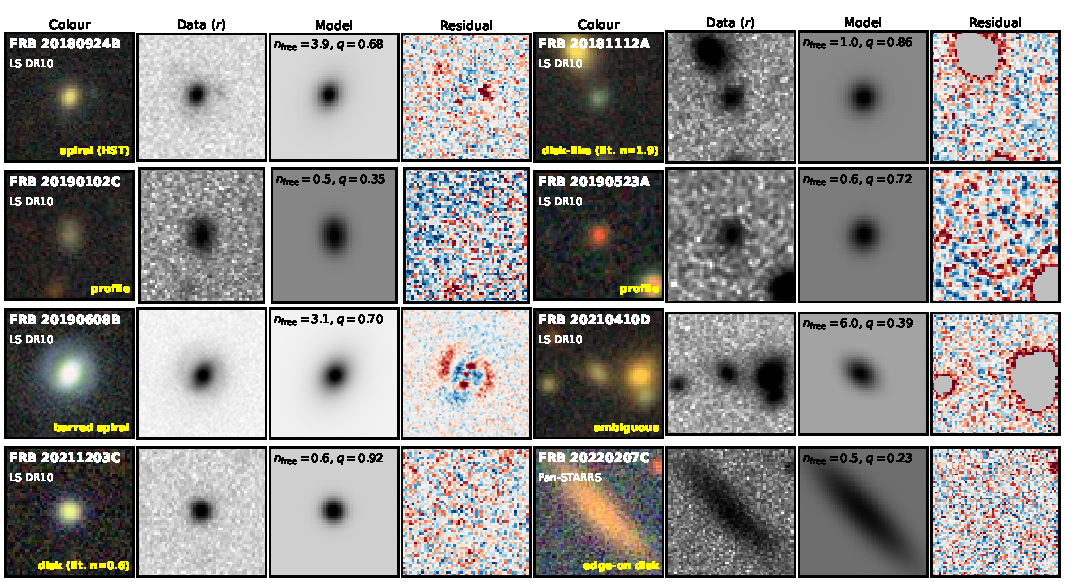
\includegraphics[width=\textwidth]{galaxy/gallery_1.pdf}\\[2pt]
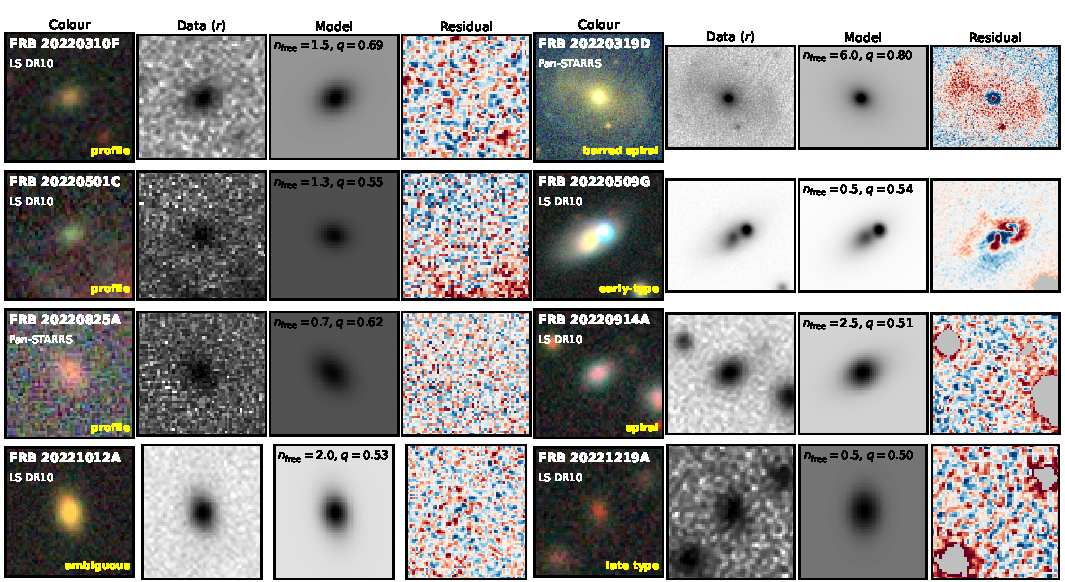
\includegraphics[width=\textwidth]{galaxy/gallery_2.pdf}
\caption{The hosts of Table~\ref{tab:disk_evidence}. For each host, from left
to right: color image (LS or Pan-STARRS), $r$-band image used in our fit, the
PSF-convolved \texttt{GALFIT} model, and the residual (masked pixels in grey).
The model panel gives $n_{\rm free}$ and the adopted $q$, and the color panel
the class of Table~\ref{tab:disk_evidence}. Spiral arms and bars appear in the
residuals of the resolved hosts.}
\label{fig:gallery1}
\end{figure}

\begin{figure}[H]
\centering
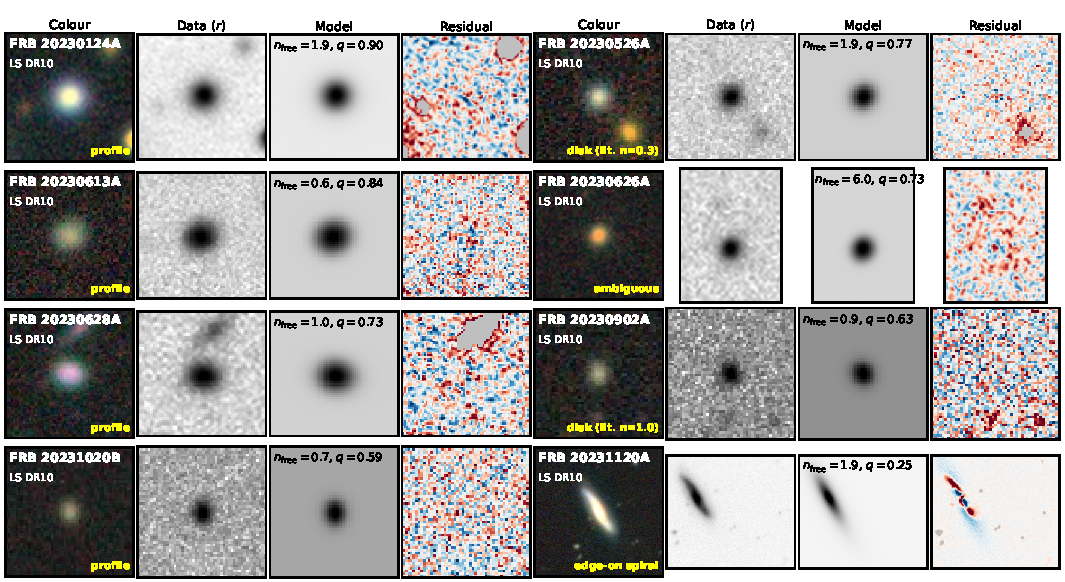
\includegraphics[width=\textwidth]{galaxy/gallery_3.pdf}\\[2pt]
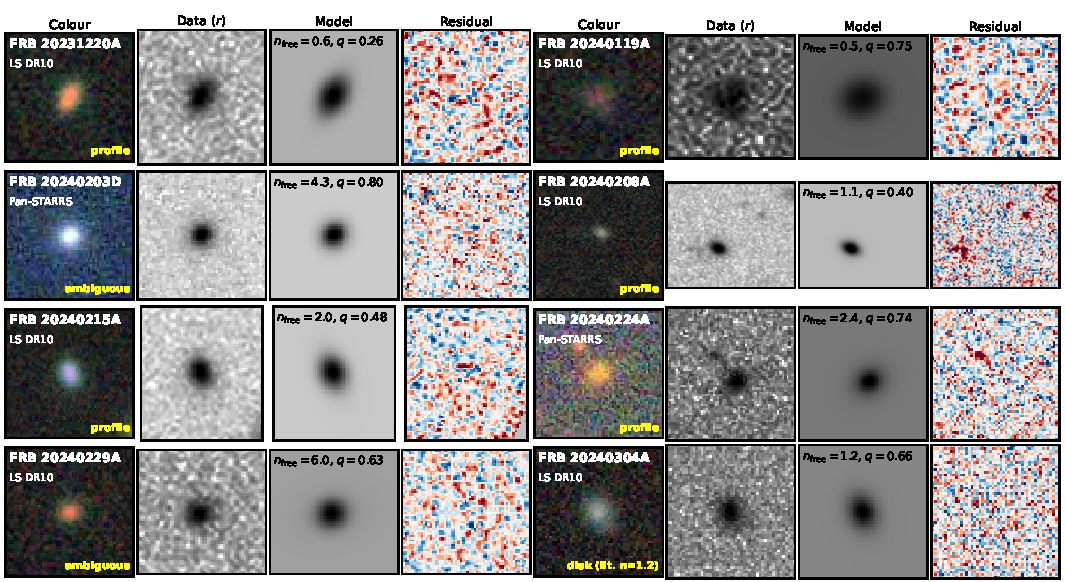
\includegraphics[width=\textwidth]{galaxy/gallery_4.pdf}
\caption{Continuation of Figure~\ref{fig:gallery1}.}
\label{fig:gallery2}
\end{figure}
 
\section{Robustness of the Inclination Measurements} \label{app:robust}
 
\subsection{Choice of $q_0$} \label{app:q0}
 
We repeat our analysis for $q_0 = 0.10$, 0.15, and 0.25, applying the cut
$q > q_0$ to both samples (Figure~\ref{fig:q0} and Table~\ref{tab:q0}). For
$q_0 \leq 0.15$, FRB 20240201A ($q = 0.18$) re-enters the sample, and for
$q_0 = 0.25$, the four hosts with $0.2 < q \leq 0.25$ are removed (FRBs
20220207C, 20231120A, 20231210F, and 20240213A). For $0.10 \leq q_0 \leq 0.20$, the
results are nearly unchanged. For $q_0 = 0.25$, the probabilities decrease,
since the removed hosts are among the most inclined in our sample, but no
test indicates a significant difference.
 
\begin{figure}[H]
\centering
\includegraphics[width=\textwidth]{figC_q0.pdf}
\caption{CDFs of $\cos i$ for the FRB hosts (red) and the control sample
(blue) for four values of $q_0$. In each panel, the shaded region shows the
68\% bound of random samples of the same size as the FRB sample, and the
dashed line a uniform distribution. Each panel gives $q_0$ and the AD
$p_{\rm m}$.}
\label{fig:q0}
\end{figure}
 
\startlongtable
\begin{deluxetable}{cccccc}
\tabletypesize{\footnotesize}
\tablewidth{0pt}
\tablecaption{Sensitivity to $q_0$\label{tab:q0}}
\tablehead{
\colhead{$q_0$} & \colhead{$N_{\rm FRB}$} & \colhead{$N_{\rm control}$} &
\colhead{AD} & \colhead{MW (two-sided)} & \colhead{MW (one-sided)}}
\startdata
0.10 & 57 & 24{,}976 & 0.57 & 0.43 & 0.21 \\
0.15 & 57 & 24{,}870 & 0.59 & 0.46 & 0.24 \\
0.20 & 56 & 24{,}450 & 0.54 & 0.46 & 0.23 \\
0.25 & 52 & 23{,}699 & 0.21 & 0.17 & 0.09 \\
\enddata
\tablecomments{Values are $p_{\rm m}$, as in Table~\ref{tab:control_robust}.}
\end{deluxetable}
 
\subsection{Measurement Uncertainties} \label{app:errors}
 
To include measurement uncertainties, we repeat our tests for 2{,}000
realizations. In each, we draw the axis ratio of every host from a Gaussian
of width $\sigma_q$ (Section~\ref{sec:inclination}), redrawing values outside
$q_0 < q \leq 1$, convert it to an inclination, and add a Gaussian scatter of
\ang{5} (Equation~\ref{eq:InclinationSystematic}), reflecting values beyond
\ang{0} and \ang{90}. The same \ang{5} scatter is applied to every galaxy in
the control sample, so that both samples are treated alike. Across these
realizations, the AD test gives a median $p_{\rm m}$ of 0.50 (16th--84th
percentile range 0.29--0.74), and the two-sided and one-sided MW tests give
0.43 (0.26--0.66) and 0.21 (0.13--0.33), respectively. None of the
realizations gives $p_{\rm m} < 0.05$ in the AD or two-sided MW test, and only
0.4\% do in the one-sided MW test. Measurement uncertainties therefore do not
change our conclusions.

\section{The Role of the PSF} \label{app:psf}

\subsection{Fits With and Without the PSF} \label{app:nopsf}

To isolate the effect of the PSF, we refit all 56 hosts without PSF
convolution, using both \texttt{GALFIT} and \texttt{AstroPhot} and keeping all
other settings of our adopted fits; restoring the PSF in this setup reproduces
the adopted fits exactly. Without the PSF, $q$ increases for 55 of the 56 hosts
in both codes, by a median of 0.11, and the two codes agree closely with each
other (median difference in $q$ below 0.001). The increase is larger for hosts
smaller than the PSF (median $\Delta q = 0.18$ for the 26 hosts with
$R_e/{\rm FWHM} < 1$, compared with 0.08 for the other 30), as expected from
PSF circularization. As a result, the median inclination falls from
\ang{51.3} to \ang{38}, 32 of the 56 hosts move into the most face-on bin, and
every test differs from the control sample at $p_{\rm m} \leq 10^{-4}$
(Table~\ref{tab:fitvariants}). PSF-convolved \texttt{AstroPhot} fits, in
contrast, give the same result as \texttt{GALFIT}. For the 22 hosts shared
with \citet{Bhardwaj2024}, our fits without the PSF reproduce their published
inclinations (median difference \ang{0.0}, RMS \ang{3.4}), while our
PSF-convolved fits are a median \ang{9} more inclined. Together, these results
indicate that the face-on excess found by \citet{Bhardwaj2024} is mainly a
consequence of fitting without the PSF, which is natural for resolved galaxies
but becomes important for the many FRB hosts that are only marginally resolved
in ground-based imaging.

\startlongtable
\begin{deluxetable*}{lcccccc}
\tabletypesize{\footnotesize}
\tablecolumns{7}
\tablewidth{0pt}
\tablecaption{Inclination tests with and without the PSF\label{tab:fitvariants}}
\tablehead{
\colhead{Axis ratios} & \colhead{$N_{\rm FRB}$} & \colhead{Median $i$} &
\colhead{Bins} & \colhead{AD} & \colhead{MW (two-sided)} & \colhead{MW (one-sided)}}
\startdata
\texttt{GALFIT}, PSF-convolved (adopted) & 56 & \ang{51.3} & 14, 19, 10, 13 & 0.54 & 0.46 & 0.23 \\
\texttt{AstroPhot}, PSF-convolved & 56 & \ang{53.2} & 13, 18, 8, 17 & 0.44 & 0.99 & 0.50 \\
\texttt{GALFIT}, no PSF & 56 & \ang{38.0} & 32, 13, 6, 5 & $\leq 10^{-4}$ & $\leq 10^{-4}$ & $\leq 10^{-4}$ \\
\texttt{AstroPhot}, no PSF & 56 & \ang{38.1} & 31, 14, 6, 5 & $\leq 10^{-4}$ & $\leq 10^{-4}$ & $\leq 10^{-4}$ \\
\cutinhead{Hosts shared with \citet{Bhardwaj2024}}
This work & 22 & \ang{52.8} & 5, 7, 4, 6 & 0.96 & 0.85 & 0.43 \\
\citet{Bhardwaj2024} & 22 & \ang{42.5} & 11, 7, 2, 2 & 0.004 & 0.004 & 0.003 \\
\enddata
\tablecomments{Values are $p_{\rm m}$, as in Table~\ref{tab:control_robust},
against the adopted control sample. Bins give the number of hosts in each
quartile of the control sample's $\cos i$ distribution, from face-on to
edge-on. With 10{,}000 random draws, the smallest possible $p_{\rm m}$ is
$10^{-4}$.}
\end{deluxetable*}

\subsection{Imaging of the Hosts Shared with \citet{Bhardwaj2024}} \label{app:images}

Of the 22 hosts shared with \citet{Bhardwaj2024}, 18 were fit on images from
the same survey in both studies (11 from LS DR10 and 7 from Pan-STARRS), and
none uses LS DR9. For the remaining four (FRBs 20190714A, 20210320C, 20220509G,
and 20220914A), \citet{Bhardwaj2024} used Pan-STARRS, while we use LS DR10. To
test whether the choice of survey matters, we refit these four hosts on
Pan-STARRS images with our pipeline. With PSF convolution, the Pan-STARRS
inclinations agree with our LS values to within \ang{4} for three hosts. The
fourth, FRB 20210320C, is nearly round and smaller than the PSF, so its
inclination is very sensitive to $q$, and it is \ang{12} more face-on in
Pan-STARRS (\ang{35} compared with \ang{47}). Without the PSF, the same
Pan-STARRS images give \ang{51}, \ang{28}, and \ang{45} for the three compact
hosts, within \ang{1} of the values of \citet{Bhardwaj2024}, and the
well-resolved FRB 20220509G ($R_e \approx 6\farcs6$) agrees with their value
when fit with the PSF (\ang{58} compared with \ang{60}). The choice of survey
therefore has a small effect compared with that of the PSF.

\subsection{Hosts Shared with \citet{marnoch2026}} \label{app:marnoch}

\citet{marnoch2026} also fit PSF-convolved single-S\'ersic profiles with
\texttt{GALFIT}, but on deeper VLT/FORS2 imaging with a smaller PSF. For the
20 hosts in both samples, our axis ratios agree closely with theirs
($r_S = 0.86$, median $|\Delta q| = 0.03$). Four hosts differ by more than
three times the median absolute deviation. Three of these, FRBs 20230902A,
20220501C, and 20190102C, are smaller than our PSF ($R_e/{\rm FWHM} = 0.38$,
0.52, and 0.65), and the smallest shared host, FRB 20230902A, shows the
largest difference ($\Delta q = +0.24$). For such hosts, even a PSF-convolved
fit to ground-based imaging retains some sensitivity to the PSF, and the
sharper FORS2 imaging may give the more reliable axis ratio. For the fourth,
FRB 20190608B, \citet{marnoch2026} fit a bulge and a disk, whereas we fit a
single S\'ersic profile. Without these four hosts, $r_S = 0.99$ and the median
$|\Delta q| = 0.02$. When the PSF is modeled, archival imaging therefore
recovers the axis ratios measured in deeper, sharper imaging for all but the
smallest hosts. Our values of DM$_{\rm host}$ for the shared hosts also track
theirs closely ($r_S = 0.99$), with a median offset of 62~pc~cm$^{-3}$ in the
host rest frame. In the observer frame the offset is nearly independent of
redshift (median 48~pc~cm$^{-3}$), and it mostly reflects their subtraction
of a 40~pc~cm$^{-3}$ Milky Way halo term, with small differences in the
adopted DM$_{\rm cosmic}$ making up the rest. To combine the two samples, we
therefore add this median offset, scaled by $(1+z)$, to their values for the
hosts not in our sample. The 69 unique hosts then give a weaker correlation
between DM$_{\rm host}$ and $q$ that is not significant ($r_S = -0.21$,
$p = 0.08$; $r_S = -0.22$, $p = 0.07$ with their values for the shared
hosts), compared with $r_S = -0.43$ ($p = 0.011$) for their sample alone
(Appendix~\ref{app:stats}).

\section{Foreground Halos and Robust Correlations} \label{app:halo}

\subsection{Foreground Halo Contribution} \label{app:fg}

Galaxy halos intersected by the sightline add to the observed DM, and any part
of this contribution not included in $\widetilde{\rm DM}_{\rm cosmic}$ is
assigned to DM$_{\rm host}$. We estimate it following Appendix~B of
\citet{Bhardwaj2025} for the 49 of our 55 hosts with spectroscopic redshifts
that lie in the LS DR9 or DR10 footprint. For each FRB, we select galaxies
within \ang{0.5} from the LS photometric-redshift catalog
\citep{Dey2019, Zhou2021}, using spectroscopic redshifts from DESI DR1
\citep{DESIDR1}, SDSS DR17 \citep{Abdurrouf2022}, and the Siena Galaxy Atlas
\citep{Moustakas2023} where available. We estimate stellar masses from the
$g-r$ color \citep{Bell2003}, convert them to halo masses with the relation of
\citet{Moster2013}, and integrate a modified NFW gas profile
\citep{ProchaskaZheng2019}, with concentrations from \citet{Dutton2014}, along the
sightline. We make three small changes to this procedure, which otherwise let a
few bright galaxies with uncertain photometric redshifts dominate the total: we
$k$-correct the photometry by interpolating the observed spectral energy
distribution, weight each galaxy by the probability that it lies in front of
the host, and discard galaxies with only photometric redshifts and
$M_r < -24$. Given the same inputs, our calculation reproduces the halo
contributions computed with the code of \citet{Bhardwaj2025} for the galaxies
intersected by FRB 20240114A to within 6\%.

The foreground contribution in the host rest frame has a median of
58~pc~cm$^{-3}$ (84th percentile 195~pc~cm$^{-3}$), exceeds 100~pc~cm$^{-3}$ for
15 hosts, and is a median 24\% of DM$_{\rm host}$. Part of it, however, is
already included in $\widetilde{\rm DM}_{\rm cosmic}$, which accounts for the
average halo gas along random sightlines. Repeating the calculation for two
random sightlines \ang{0.75} from each FRB gives a median of 43~pc~cm$^{-3}$,
comparable to that of the FRB sightlines, and subtracting the full
contribution makes DM$_{\rm host}$ negative for six hosts. We therefore
consider both the full contribution and its excess over the random
sightlines. The foreground
contribution is uncorrelated with $q$ ($r_S = 0.14$, $p = 0.33$), as expected
since it does not depend on the orientation of the host, and subtracting
either version leaves the correlation of DM$_{\rm host}$ with $q$ unchanged
(Table~\ref{tab:robustcorr}).

\subsection{Correlation Statistics} \label{app:stats}

Table~\ref{tab:robustcorr} lists, for each property, the Spearman $r_S$ with
its 95\% bootstrap interval \citep{Efron1979} and $p$-value, Kendall's $\tau$
\citep{Kendall1938}, and two further checks. The Spearman $p$-value is the
probability of a correlation at least as strong as observed if the two
quantities are independent; it follows from
$t = r_S\sqrt{(N-2)/(1-r_S^2)}$, which has a Student $t$ distribution with
$N-2$ degrees of freedom, so that the $|r_S|$ needed for $p < 0.05$ falls from
0.40 for $N = 24$ to 0.27 for $N = 55$. First, to test whether a few hosts
drive or hide a correlation, we recompute $r_S$ for every subset with one,
two, or three hosts removed (27{,}775 subsets for $N = 55$). Second, since
rank correlations test only for a monotonic trend, we compare the
distributions of each property in the more face-on half of the hosts ($q$
above the median) and the more edge-on half with the two-sample AD test, using
10{,}000 permutations to obtain $p_{\rm AD}$. No DM$_{\rm host}$ subsample
reaches $p < 0.05$ in either test, for any subset with up to three hosts
removed. The extinction of the older stellar population is the only property
that differs between the two halves ($p_{\rm AD} = 0.005$).

The table also lists DM$_{\rm host}$ for the sample of \citet{marnoch2026}
and for its union with ours. Their correlation is robust within their sample:
it remains at $p < 0.05$ after removing any one or two hosts and in 99\% of
cases with three removed, and the AD test also finds a difference between the halves
($p_{\rm AD} = 0.03$). In the combined sample, with their DM$_{\rm host}$
values shifted onto our definition (Appendix~\ref{app:marnoch}), the
correlation weakens to $r_S = -0.21$ or $-0.22$ ($p = 0.08$ or 0.07),
depending on which measurements are used for the shared hosts. The AD test
gives $p_{\rm AD} = 0.04$ to 0.12, and 12\% to 17\% of the subsets with three
hosts removed reach $p < 0.05$. Part of the remaining trend comes from four
hosts of \citet{marnoch2026}, none of them in our sample, with $q < q_0$,
which they assign $i = \ang{90}$ and which our selection would exclude.
Without them, the combined sample gives $r_S = -0.16$ ($p = 0.20$) or
$-0.17$ ($p = 0.17$) for the two choices, with fewer than 1\% of the
three-host subsets reaching $p < 0.05$, and their sample alone gives
$r_S = -0.36$ ($p = 0.05$; $p_{\rm AD} = 0.18$). A weak trend in the
combined sample therefore cannot be excluded, but it is much weaker than in
the sample of \citet{marnoch2026} alone and is not significant.

\startlongtable
\begin{deluxetable*}{lcccccccc}
\tabletypesize{\scriptsize}
\setlength{\tabcolsep}{3pt}
\tablecolumns{9}
\tablewidth{0pt}
\tablecaption{Correlations with host axis ratio\label{tab:robustcorr}}
\tablehead{
\colhead{Property} & \colhead{$N$} & \colhead{$r_S$} & \colhead{95\% CI} & \colhead{$p$} &
\colhead{$\tau$ ($p$)} & \colhead{$p_{\rm AD}$} &
\colhead{JK$_1$} & \colhead{JK$_3$ ($f_{p<0.05}$)}}
\startdata
DM$_{\rm host}$ & 55 & $-0.06$ & $[-0.32, +0.20]$ & 0.64 & $-0.04$ (0.63) & 0.18 & $[-0.12, -0.04]$ & $[-0.21, +0.02]$ (0) \\
\quad foreground removed & 49 & $-0.04$ & $[-0.33, +0.25]$ & 0.78 & $-0.03$ (0.76) & 0.32 & $[-0.09, +0.00]$ & $[-0.20, +0.09]$ (0) \\
\quad foreground excess removed & 49 & $-0.07$ & $[-0.35, +0.21]$ & 0.62 & $-0.05$ (0.58) & 0.31 & $[-0.13, -0.03]$ & $[-0.23, +0.06]$ (0) \\
\quad $m_r < 21$ & 45 & $-0.09$ & $[-0.38, +0.19]$ & 0.54 & $-0.07$ (0.52) & 0.22 & $[-0.16, -0.06]$ & $[-0.29, +0.00]$ (0) \\
\quad $n < 2$ & 46 & $-0.04$ & $[-0.32, +0.26]$ & 0.81 & $-0.02$ (0.85) & 0.58 & $[-0.10, +0.00]$ & $[-0.22, +0.08]$ (0) \\
\quad bulge fits removed & 52 & $-0.07$ & $[-0.34, +0.20]$ & 0.64 & $-0.04$ (0.64) & 0.25 & $[-0.12, -0.04]$ & $[-0.22, +0.02]$ (0) \\
$|{\rm RM}|$ & 41 & $-0.02$ & $[-0.31, +0.30]$ & 0.91 & $-0.00$ (0.99) & 0.29 & $[-0.09, +0.04]$ & $[-0.20, +0.15]$ (0) \\
Scattering time & 29 & $-0.17$ & $[-0.55, +0.27]$ & 0.39 & $-0.11$ (0.41) & 0.83 & $[-0.28, -0.07]$ & $[-0.47, +0.08]$ ($<0.01$) \\
Linear polarization & 24 & $-0.33$ & $[-0.69, +0.12]$ & 0.11 & $-0.24$ (0.10) & 0.50 & $[-0.45, -0.25]$ & $[-0.60, -0.08]$ (0.11) \\
$A_V$, old stars & 30 & $-0.46$ & $[-0.67, -0.15]$ & 0.010 & $-0.28$ (0.03) & 0.005 & $[-0.53, -0.41]$ & $[-0.61, -0.31]$ (0.97) \\
\cutinhead{DM$_{\rm host}$ in the sample of \citet{marnoch2026} (M26) and in the combined sample}
M26 & 34 & $-0.43$ & $[-0.65, -0.14]$ & 0.011 & $-0.28$ (0.02) & 0.030 & $[-0.52, -0.39]$ & $[-0.60, -0.32]$ (0.99) \\
\quad $q > q_0$ & 30 & $-0.36$ & $[-0.63, -0.02]$ & 0.052 & $-0.24$ (0.06) & 0.18 & $[-0.45, -0.29]$ & $[-0.58, -0.21]$ (0.29) \\
Combined, ours for shared & 69 & $-0.21$ & $[-0.43, +0.02]$ & 0.082 & $-0.14$ (0.09) & 0.037 & $[-0.26, -0.19]$ & $[-0.34, -0.15]$ (0.12) \\
\quad $q > q_0$ & 65 & $-0.16$ & $[-0.39, +0.08]$ & 0.20 & $-0.11$ (0.20) & 0.094 & $[-0.21, -0.13]$ & $[-0.29, -0.09]$ ($<0.01$) \\
Combined, M26 for shared & 69 & $-0.22$ & $[-0.43, +0.01]$ & 0.070 & $-0.15$ (0.07) & 0.12 & $[-0.27, -0.20]$ & $[-0.35, -0.16]$ (0.17) \\
\quad $q > q_0$ & 65 & $-0.17$ & $[-0.40, +0.07]$ & 0.17 & $-0.12$ (0.17) & 0.076 & $[-0.22, -0.14]$ & $[-0.30, -0.10]$ ($<0.01$) \\
\enddata
\tablecomments{CI is the 95\% bootstrap interval of $r_S$ (10{,}000 resamples).
$p_{\rm AD}$ compares the property distributions of the hosts with $q$ above
and below the median (10{,}000 permutations). JK$_1$ and JK$_3$ give the range
of $r_S$ over all subsets with one or three hosts removed, and $f_{p<0.05}$ the
fraction of three-host subsets that reach $p < 0.05$. Indented rows are
subsamples of the row above. ``Bulge fits removed'' excludes the three hosts
that M26 fit with a bulge component, and the $q > q_0$ rows exclude the four
hosts of M26 with $q < q_0$. ``Ours/M26 for shared'' gives the DM$_{\rm host}$
used for the 20 shared hosts, with the M26 values shifted onto our definition
(Appendix~\ref{app:marnoch}).}
\end{deluxetable*}
 

%% For this sample we use BibTeX plus aasjournalv7.bst to generate the
%% the bibliography. The sample7.bib file was populated from ADS. To
%% get the citations to show in the compiled file do the following:
%%
%% pdflatex sample7.tex
%% bibtext sample7
%% pdflatex sample7.tex
%% pdflatex sample7.tex

\bibliography{paper,new_refs}{}
\bibliographystyle{aasjournalv7}

%% This command is needed to show the entire author+affiliation list when
%% the collaboration and author truncation commands are used.  It has to
%% go at the end of the manuscript.
%\allauthors

%% Include this line if you are using the \added, \replaced, \deleted
%% commands to see a summary list of all changes at the end of the article.
%\listofchanges

\end{document}

% End of file `sample7.tex'.
